\documentclass[journal]{vgtc}                % final (journal style)
%\documentclass[review,journal]{vgtc}         % review (journal style)
%\documentclass[widereview]{vgtc}             % wide-spaced review
%\documentclass[preprint,journal]{vgtc}       % preprint (journal style)

%% Uncomment one of the lines above depending on where your paper is
%% in the conference process. ``review'' and ``widereview'' are for review
%% submission, ``preprint'' is for pre-publication, and the final version
%% doesn't use a specific qualifier.

%% Please use one of the ``review'' options in combination with the
%% assigned online id (see below) ONLY if your paper uses a double blind
%% review process. Some conferences, like IEEE Vis and InfoVis, have NOT
%% in the past.

%% Please use the ``preprint''  option when producing a preprint version
%% for sharing your article on an open access repository

%% Please note that the use of figures other than the optional teaser is not permitted on the first page
%% of the journal version.  Figures should begin on the second page and be
%% in CMYK or Grey scale format, otherwise, colour shifting may occur
%% during the printing process.  Papers submitted with figures other than the optional teaser on the
%% first page will be refused. Also, the teaser figure should only have the
%% width of the abstract as the template enforces it.

%% These few lines make a distinction between latex and pdflatex calls and they
%% bring in essential packages for graphics and font handling.
%% Note that due to the \DeclareGraphicsExtensions{} call it is no longer necessary
%% to provide the the path and extension of a graphics file:
%% 
\includegraphics{diamondrule} is completely sufficient.
%%
\ifpdf%                                % if we use pdflatex
  \pdfoutput=1\relax                   % create PDFs from pdfLaTeX
  \pdfcompresslevel=9                  % PDF Compression
  \pdfoptionpdfminorversion=7          % create PDF 1.7
  \ExecuteOptions{pdftex}
  \usepackage{graphicx}                % allow us to embed graphics files
  \DeclareGraphicsExtensions{.pdf,.png,.jpg,.jpeg} % for pdflatex we expect .pdf, .png, or .jpg files
\else%                                 % else we use pure latex
  \ExecuteOptions{dvips}
  \usepackage{graphicx}                % allow us to embed graphics files
  \DeclareGraphicsExtensions{.eps}     % for pure latex we expect eps files
\fi%

%% it is recomended to use ``\autoref{sec:bla}'' instead of ``Fig.~\ref{sec:bla}''
\graphicspath{{figures/}{pictures/}{images/}{./}} % where to search for the images
\vgtcinsertpkg
\usepackage{microtype}                 % use micro-typography (slightly more compact, better to read)
\PassOptionsToPackage{warn}{textcomp}  % to address font issues with \textrightarrow
\usepackage{textcomp}                  % use better special symbols
\usepackage{mathptmx}                  % use matching math font
\usepackage{times}                     % we use Times as the main font
\renewcommand*\ttdefault{txtt}         % a nicer typewriter font
\usepackage{cite}                      % needed to automatically sort the references
% \usepackage[backend=biber,doi=false,isbn=false,url=false,eprint=false]{biblatex}
% \addbibresource{template.bib}
\usepackage{tabu}                      % only used for the table example
\usepackage{booktabs}                  % only used for the table example
\usepackage{support-caption}
\usepackage{subcaption,subfloat}
\usepackage{minted}
\usepackage{soul}
\usepackage{placeins}

\newcommand{\makeSampleFig}{%
\begin{figure}[tb]
 \centering % avoid the use of \begin{center}...\end{center} and use \centering instead (more compact)
 \includegraphics[width=\columnwidth]{paper-count-w-2015-new}
 \caption{A visualization of the 1990--2015 data from \autoref{tab:vis_papers}. The image is from \cite{Isenberg:2017:VMC} and is in the public domain.}
 \label{fig:sample}
\end{figure}}
%% We encourage the use of mathptmx for consistent usage of times font
%% throughout the proceedings. However, if you encounter conflicts
%% with other math-related packages, you may want to disable it.

%% In preprint mode you may define your own headline. If not, the default IEEE copyright message will appear in preprint mode.
%\preprinttext{To appear in IEEE Transactions on Visualization and Computer Graphics.}

%% In preprint mode, this adds a link to the version of the paper on IEEEXplore
%% Uncomment this line when you produce a preprint version of the article 
%% after the article receives a DOI for the paper from IEEE
%\ieeedoi{xx.xxxx/TVCG.201x.xxxxxxx}

%% If you are submitting a paper to a conference for review with a double
%% blind reviewing process, please replace the value ``0'' below with your
%% OnlineID. Otherwise, you may safely leave it at ``0''.
\onlineid{0}

%% declare the category of your paper, only shown in review mode
\vgtccategory{Research}
%% please declare the paper type of your paper to help reviewers, only shown in review mode
%% choices:
%% * algorithm/technique
%% * application/design study
%% * evaluation
%% * system
%% * theory/model
\vgtcpapertype{please specify}

%% Paper title.
\title{Semi-Supervised Semantic Annotator (S3A): Toward Efficient Semantic Image Labeling}

%% This is how authors are specified in the journal style

%% indicate IEEE Member or Student Member in form indicated below
\author{Nathan Jessurun, Daniel E. Capecci, Olivia P. Paradis, Damon Woodard, Navid Asadizanjani}
\authorfooter{
%% insert punctuation at end of each item
\item
 All authors are with the Florida Institute for Cybersecurity Research (FICS) at the Univeristy of Florida. E-mail: {njessurun | dcapecci | paradiso}@ufl.edu, {dwoodard | nasadi}@ece.ufl.edu.
}

%other entries to be set up for journal
\shortauthortitle{Biv \MakeLowercase{\textit{et al.}}: Global Illumination for Fun and Profit}
%\shortauthortitle{Firstauthor \MakeLowercase{\textit{et al.}}: Paper Title}

%% Abstract section.
\abstract{Most semantic image annotation platforms suffer severe bottlenecks when handling large images, complex regions of interest, or numerous distinct foreground regions in a single image. We have developed the Semi-Supervised Semantic Annotator (S3A) to address each of these issues and facilitate rapid collection of ground truth pixel-level labeled data. Such a feat is accomplished through a robust and easy-to-extend integration of arbitrary python image processing functions into the semantic labeling process. Importantly, the framework devised for this application allow easy visualization and machine learning prediction of arbitrary formats and amounts of per-component metadata. To our knowledge, the ease and flexibility offered are unique to S3A among all open-source alternatives. S3A is available through pypi.org (\href{https://pypi.org/project/s3a/}{https://pypi.org/project/s3a/}) and GitLab (\href{https://gitlab.com/ficsresearch/s3a}{https://gitlab.com/ficsresearch/s3a}).%
} % end of abstract

%% Keywords that describe your work. Will show as 'Index Terms' in journal
%% please capitalize first letter and insert punctuation after last keyword
\keywords{Radiosity, global illumination, constant time}

%% ACM Computing Classification System (CCS). 
%% See <http://www.acm.org/class/1998/> for details.
%% The ``\CCScat'' command takes four arguments.

\CCScatlist{ % not used in journal version
 \CCScat{K.6.1}{Management of Computing and Information Systems}%
{Project and People Management}{Life Cycle};
 \CCScat{K.7.m}{The Computing Profession}{Miscellaneous}{Ethics}
}

%% A teaser figure can be included as follows
\teaser{
  \centering
  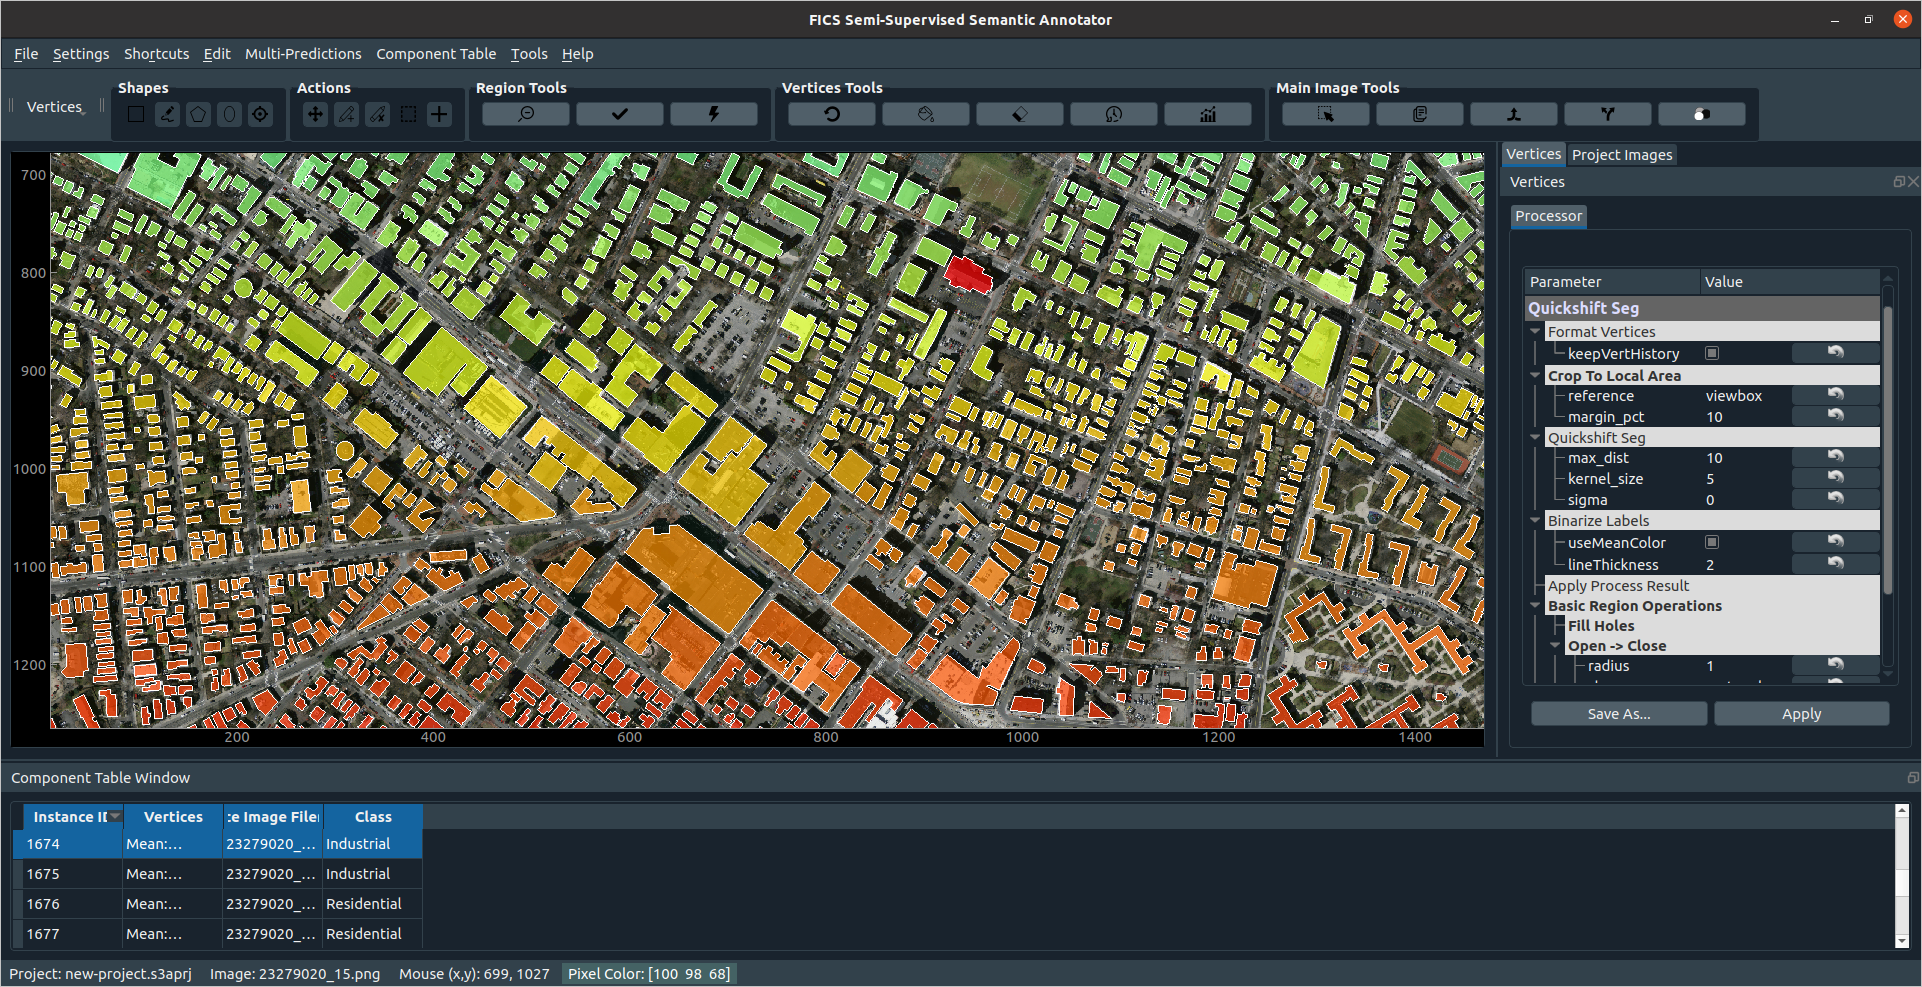
\includegraphics[width=\linewidth]{figures/appOverview}
  \caption{S3A's interface. The main view consists of an image to annotate, a component table of prior annotations, and a toolbar which changes functionality depending on context. Image under annotation retrieved from \url{https://www.kaggle.com/bulentsiyah/semantic-drone-dataset}.}
  \label{fig:teaser}
}

%% Uncomment below to disable the manuscript note
%\renewcommand{\manuscriptnotetxt}{}

%% Copyright space is enabled by default as required by guidelines.
%% It is disabled by the 'review' option or via the following command:
% \nocopyrightspace

%%%%%%%%%%%%%%%%%%%%%%%%%%%%%%%%%%%%%%%%%%%%%%%%%%%%%%%%%%%%%%%%
%%%%%%%%%%%%%%%%%%%%%% START OF THE PAPER %%%%%%%%%%%%%%%%%%%%%%
%%%%%%%%%%%%%%%%%%%%%%%%%%%%%%%%%%%%%%%%%%%%%%%%%%%%%%%%%%%%%%%%%

\begin{document}

%% The ``\maketitle'' command must be the first command after the
%% ``\begin{document}'' command. It prepares and prints the title block.

\maketitle

\section{Introduction}
Labeled image data is essential for tuning and evaluating the performance of machine learning applications.
Such labels are typically defined with approximate enclosing shapes (i.e. simple polygons or parametric shapes), which tend to misrepresent more complex components.
% While this streamlines the labeling process, it misrepresents more complex components.
% When high accuracy is required, labels must be specified at the pixel-level – a process known as segmentation labeling or semantic segmentation.
% A detailed description of this process is explained in \cite{chengSurveyAnalysisAutomatic2018}.

% However, a wide variety of applications require pixel-level accuracy, ranging from hardware assurance to medical imaging.
Alternatively, semantic segmentation is a technique providing pixel-level accuracy which avoids poor foreground representation~\cite{chengSurveyAnalysisAutomatic2018}.
One such field applying this method include Bill-of-Material (BoM) extraction. This BoM, or list of all surface-mount devices (SMDs) on a printed circuit board (PCB) surface, can be generated from optical images of a board under test. Next, it can be compared against a reference design to detect likely counterfeit, tampered, or defective SMDs~\cite{paradis2020color,azhaganReviewAutomaticBill2019}. To create such a BoM using optical data alone, it is crucial that detected SMDs use segmentation masks that are representative of structures such as pins, solder flow, and more. This is the only way the collected data will remain indicative of true BoM properties. An example annotation is shown in \autoref{fig:pcb}

\makePcbFig

Beyond PCB analysis, semantic segmentation is important in several other domains including quality control during manufacturing \cite{fergusonDetectionSegmentationManufacturing2018,anagnostopoulosComputerVisionApproach2001,anagnostopoulosHighPerformanceComputing2002}, manuscript restoration / digitization \cite{gatosSegmentationfreeRecognitionTechnique2004,kesimanNewSchemeText2016,jainTextSegmentationUsing1992,taxtSegmentationDocumentImages1989,fujisawaSegmentationMethodsCharacter1992}, and effective patient diagnosis \cite{seifertSemanticAnnotationMedical2010,rajchlDeepCutObjectSegmentation2017,yushkevichUserguided3DActive2006,iakovidisRatsnakeVersatileImage2014}.
In all these cases, imprecise annotations severely limit the development of automated solutions and can decrease the accuracy of standard trained segmentation models.

Quality semantic segmentation is difficult due to a reliance on large, high-quality datasets, which are often created by manually labeling each image.
Manual annotation is error-prone, costly, and greatly hinders scalability.
Several tools have been proposed to alleviate the burden of collecting ground-truth labels for semantic segmentation~\cite{BestImageAnnotation}.
% The more commonly used applications are listed in \cite{BestImageAnnotation}.
Unfortunately, existing tools are heavily biased toward lower-resolution images with few regions of interest (ROI) (\autoref{fig:sampleSegData}).
While this may not be an issue for some datasets, such assumptions are \emph{crippling} for high-fidelity images with hundreds of annotated ROIs (\autoref{fig:bees}) \cite{Ladicky_whatWhereCombiningCRFs,Wang_multiLabelImageAnnotation}.
% This scenario is represented in Figure~\ref{fig:bees} but can occur in multiple of the domains previously listed.
% Especially when each region can be arbitrarily complex, the software will enter a non-responsive state where no annotation can be performed.

\makeSampleSegFig
\makeBeesFig

% A potential workaround is to bootstrap machine learning models through transfer learning on a similar dataset and applying them on the current dataset.
% Manual supervision is then only required to verify the results are correct and make adjustments accordingly.
% While this approach is valid when existing datasets match the desired segmentation properties, it also means transfer learning is ineffective when training on novel data or image properties.
% Moreover, transfer learning is effective in assisting ground truth collection only when a sufficient data repository has already been gathered against which to validate network training \cite{opbroekTransferLearningImproves2015,weissSurveyTransferLearning2016}.

% Even after models are trained, it can be greatly beneficial to explore edge cases and pre/post-processing techniques while supervising the ground truth collection procedure.
%Toward this end, 
S3A circumvents these pitfalls by providing deep customization of the annotation workflow at both a granular and high level.
% To the best of our knowledge, it is the only application with this capability at both a granular and high level.
Arbitrary Python functions can be seamlessly integrated into the processing workflow, and every algorithm developed within S3A can be accessed in a headless (i.e. automated or scripted) manner independent of the GUI.

In this paper, we present significant improvements to the fundamentals of S3A as previously introduced in \cite{jessurunComponentDetectionEvaluation2020}.
% Our revisions presented in this work are significant improvements to the previous publication's future work.
% In this paper, we present the core components of the S3A processing framework and labeling suite.
This includes live app-level property customization, real-time algorithm modification, and feedback, region prediction assistance, constrained component table editing based on allowed data types, a multitude of data export formats, and a highly adaptable set of plugin interfaces for application-specific extensions to S3A.
We also note the potential impact on the image processing community improving labeling speed, accuracy, and multiple insertion points for algorithm feedback.
Beyond software improvements, these features play significant roles in bridging the gap between human annotation efforts and scalable, automated segmentation methods \cite{Branson_humansInLoop}.
\section{Application Features}

\subsection{Motivation}\label{sec:motivation}
All application features are driven by the following objectives:

Metadata should have significance rather than be treated as an afterthought

Large images should have minimal impact on the annotation workflow

Similarly, a multitude of regions or significant region complexity should not penalize the annotator.

Why were these chosen? Cite some works about how 

\subsection{Processing Framework}\label{sec:procFramework}
At the root of S3A's functionality and configurability lies its adaptive processing framework. Functions exposed within S3A are thinly wrapped using a Process structure responsible for parsing signature information to provide documentation, parameter information, and more to the UI. Hence, all graphical depictions are abstracted beyond the concern of the user while remaining trivial to specify (but can be modified or customized if desired). As a result, incorporating additional application functionality requires few lines of code. An example of this wrapping mechanism is depicted in \autoref{fig:atomicProc}. Processes interface with PyQtGraph parameters to gain access to data-customized widget types and more (\href{https://github.com/pyqtgraph/pyqtgraph}{https://github.com/pyqtgraph/pyqtgraph}).

\makeAtomicProcFig

Such processes can also be arbitrarily nested and chained. This feature is critical for developing hierarchical image processing models, an example of which is shown in \autoref{fig:nestedProc}. This framework is used for all image and region processing within S3A.

\makeNestedProcFig

\subsubsection{Image Processes}
Image processes are a special case of the generalized paradigm described in \autoref{sec:procFramework}, since they are also capable of depicting stage-by-stage results and analytics after an operation has taken place. This feature is especially useful for determining the failure point in a chain of algorithms, allowing a user to quickly determine the most effective set of parameters for a given set of inputs. Moreover, image processes can be windowed at several levels (image, viewbox, component, and roi) to drastically improve performance in high-resolution inputs with sparsely populated foregrounds.


\hl{figure of region analytics}

Consider the case where \hl{Use case for using region analytics to determine point of failure}

\subsubsection{Impact}
Of the existing open source tools for semantic annotation, few allow users to insert custom algorithms to perform the task at hand. Fewer still provide a building-block framework in which user functions can be mixed and matched as needed to produce optimal results. Hence, users are not required to uploading turnkey algorithmic solutions. Instead, they can hierarchically combine granular stages based on dynamic feedback to iteratively converge on a preferable processing tactic. As a result, datasets can receive annotations far more quickly and more accurately, improving the performance of subsequent trained models.

\subsection{Model-Based Region Proposal}

Beyond single region editing, S3A also exposes a framework for region-proposal mechanisms leveraging either traditional computer vision or machine learning techniques. With minimal scaffolding, users with existing algorithms or network architectures can insert their technique directly into the annotation process and receive fine-tuned control over all modifiable input parameters.

Since S3A utilizes a project structure, such predictions can be applied ahead of time to alternate images in the same project if desired. As a result, future project images can potentially be completed by this prediction mechanism with even less manual effort. The ultimate goal of such an integration is to gradually convert the task of manual image \emph{annotation} to that of annotation \emph{verification}, which can be completed much more rapidly.

\subsubsection{Impact}
Unlike alternatives, S3A allows control of region proposal at both local and global areas. Thus, windowing-based approaches to region proposal can be incorporated without requiring image stitching, cropping, or similar preprocessing directives. This increases the flexibility and applicability of techniques which otherwise could not be applied to unprocessed, large images.

\subsection{Component Table}

Arbitrary metadata can be logged with each component as specified by a table configuration. Delegates for this metadata are automatically inferred, meaning dropdowns, spinboxes, checkboxes, and more are automatically integrated into the component table based on the default values specified. If no metadata is required, the user can simply rely on the default configuration which only records region boundary information. Data types are inferred by the default value for the field or can be manually specified. These capabilities are unique to S3A, as most other software only allows text-based metadata tags with minimal validation.

Furthermore, each delegate type can be filtered by specifying a range of allowable values to appear in the annotated image. In this manner, users can focus directly on the properties of most importance if they desire, and continue annotating as normal afterward. An example of this is shown in Fig \ref{fig:standFilter}, where an active filter for only a \texttt{Standing} posture allows users to quickly ensure all standing (not walking, sitting, etc.) individuals are identified.

\makeStandFilterFig

\subsubsection{Impact}
Human-annotated datasets inevitably accrue errors, either through misinterpretation or mistaken inputs \cite{Dai_crowdSourceWorkflows,Russakovsky_humanCollabAnnotation2015}. Simple techniques such as using dropdowns instead of raw text entries, limitations on integer/float labels, and related control techniques can prevent such errors from occurring early on. Since these are directly based on minimal user specifications, S3A as an annotation platform inherently maintains a level of integrity in collected attributes and metadata. An example of this is shown in \autoref{fig:boundCheck}, which indicates the limits set by a user's field configuration do not allow negative values.

\makeBoundCheckFig

\subsection{Plugins for User Extensions}
\autoref{sec:procFramework} briefly described how custom user functions are easily be wrapped within a process, exposing its parameters within S3A in a GUI format. A rich plugin interface is built on top of this capability, in which custom functions, table field predictors, default action hooks, and more can be directly integrated into S3A. In all cases, only a few lines of code are required to achieve most integrations between user code and plugin interface specifications.

\subsubsection{General Plugins}
The core plugin infrastructure consists of a function/property registration mechanism and an interaction window which shows them in the UI. As such, arbitrary user functions can be `registered` in one line of code to a plugin, where it will be effectively exposed to the user within S3A. The example from \autoref{fig:atomicProc} is shown again here, but integrated into the main application. In this case, it is appended to a list of miscellaneous functions, which are managed by a plugin provided for this purpose. Note that an extra function parameter, \texttt{win}, is optional and gives the function access to the running application.

\makeCustomMiscFuncFig

\subsubsection{Table Field Plugins}

To better facilitate prediction and handling of important metadata, any table field can have one or more associated table field plugins. This interface gives the user hooks into common component-related application hooks such as drawing on the image, making a component selection, accepting a region, and more. In this manner, an arbitrary number of table field plugins can register to application actions and fully populate a table row with minimal required effort.

\subsubsection{Impact}
Plugin features are heavily oriented toward easing the process of automation both for general annotation needs and niche datasets. In either case, incorporating existing library functions is converted into a trivial task directly resulting in lower annotation and higher labeling accuracy.

\subsection{Export Formats}
An I/O interface is provided which allows data collected through S3A to be communicated in arbitrary formats, ranging from CSV to JSON to labeled bitmaps. These are also easily extendable by users who require customized formatting.

Among these options, one export provides cutouts of each individual component for easier machine learning model training. These cutouts can be scaled to a uniform size (e.g. 500x500 pixels) to cater to networks requiring a fixed input layer width. Hence, images which can be intelligently subdivided into smaller segmentation challenges can be treated independently of the whole image if desired. An exmaple of such an export format is shown in \autoref{fig:cropExports}

\makeCropExportsFig

\subsubsection{Impact}
S3A was designed with ease of adoption and integration in mind from the beginning. Multiple export formats lower this entry barrier, and ensure multiple domains can leverage its provided data. Moreover, as mentioned in \autoref{sec:motivation}, another major goal during the creation of this software was to elevate the status of metadata to fully support its prediction, validation, and more. Hence, defining export formats that prioritize in this manner will hopefully motivate conversations about their potential importance and integration into existing annotation platforms.


\subsection{Reconfigurability}
Our previous work \cite{jessurunComponentDetectionEvaluation2020} described the idea of customizable application and color scheme behavior, a feature which has been significantly updated at present.

\subsubsection{Persistent Customized States}
Currently, any configuration of parameters can be saved in an intuitive, human-readable format. This can in turn be loaded or specified in a startup configuration as needed.

\subsubsection{Color Schemes}
Notably, S3A allows the user to freely select which table column should represent a component's color when overlaid on the input image. Depending on user goals, they have the option of displaying the component's ID, class, or any custom field as they see fit. This allows users to visually evaluate common characteristics of their data with minimal effort. An example of this is shown in \autoref{fig:reconfig}. The availability of both linear and set-wise colormaps assist visualizing both continuous ranges of values (e.g. numerical fields) and selection-based values (e.g. a "Class" dropdown). Importantly, this drastically decreases the time required to quickly spot anomalies in annotated metadata during manual quality assurance review.

\makeReconfigFigs

\subsubsection{Impact}
While these features may sound irrelevant or superfluous, they provide users with shortcuts and rapid access which immensely reduces the amount of time required to complete an annotation batch. This saved time comes at no cost to output accuracy and allows users to annotate more images as a result. Hence, software improvements such as easily accessible buttons and modifiable hotkeys for custom functions directly translate to improved model performance on the collected data.
\section{Summary of High-Level Impacts}\label{sec:impacts}
%To evaluate these claims against other popular annotation software, an experiment will be carried out to annotate images exhibiting high resolution, numerous foreground regions, and high ROI complexity. Total time required to annotate the images will be compared against the resulting accuracy to show the quantitative effects of the features proposed here.
Key takeaways from \autoref{sec:appFeatures} should strongly emphasize the exploration of annotation capabilities rather than any specific software implementation. Toward this end, S3A's major contributions for annotation and ground truth collection involve meeting both skilled and novice operators at their current level, allowing them to increase the effectiveness of their time during annotation. Beyond this, S3A also supplements existing datasets by providing a unique visualization platform. Its support of dynamic peripheral data, filtering, and more allow operators to quickly hone in on what matters in the current image.

S3A also approaches the task of annotation with a greater emphasis on manual interaction. Throughout the push for increasing automated capabilities, there is still a multitude of insertion points for tweaking parameters and exploring algorithmic solution spaces. As a result, minor adjustments in a given annotation pipeline do not require a reinvention of any individual stage. Rather, subtle changes can be incorporated on an image-by-image or region-by-region basis to leverage the greatest possible output accuracy.
\section{Conclusion and Future Work}
The Semi-Supervised Semantic Annotator (S3A) is proposed to address the difficult task of pixel-level annotations of image data. For high-resolution images with numerous complex regions of interest, existing labeling software faces performance bottlenecks attempting to extract ground-truth information. Moreover, there is a lack of capabilities to convert such a labeling workflow into an automated procedure with feedback at every step. Each of these challenges is overcome by various features within S3A specifically designed for such tasks. As a result, S3A provides not only tremendous time savings during ground truth annotation, but also allows an annotation pipeline to be directly converted into a prediction scheme. Furthermore, the rapid feedback accessible at every stage of annotation expedites prototyping of novel solutions to imaging domains in which few examples of prior work exist.

\subsection{Dynamic Algorithm Builder}
Improvements are ongoing and will include a variety of powerful features. Chief among these will be an algorithm builder to allow greater flexibility with mixing and matching useful region modification stages. Consequently, the available selection of algorithms and tweaking capabilities will be drastically increased. Rather than only modifying \emph{parameter} values, users will be able to adaptively add \emph{processing stages} as well.

\subsection{Image Navigation Assistance}
Several aspects of image navigation can be incorporated to simplify  the handling of large images. For instance, a `minimap' tool would allow users to maintain a global image perspective while making local edits. Furthermore, this sense of scale aids intuition of how many regions of similar component density, color, etc. exist within the entire image.

Second, multiple strategies for annotating large images leverage a windowing approach, where they will divide the total image into several smaller pieces in a gridlike fashion. While this has its disadvantages, it is fast, easy to automate, and produces reasonable results depending on the initial image complexity \cite{Vigueras_fullCnnCornealSegmentation}. Hence, these methods would be significantly easier to incorporate into S3A if a generalized windowing framework was incorporated which allows users to specify all necessary parameters such as window overlap, size, sampling frequency, etc.


\subsection{Aggregation of Human Annotation Habits}
Several times, it has been noted that manual segmentation of image data is not a feasible or scalable approach for remotely large datasets. However, there are multiple cases in which human intuition can greatly outperform even complex neural networks, depending on the specific segmentation challenge \cite{Russakovsky_humanCollabAnnotation2015}. For this reason, it would be ideal to capture data points hinting toward this decision-making process and use this information to represent human evaluation of images at scale. This may include taking into account human labeling time per class, hesitation between clicks, relationship between shape boundary complexity and instance quantity, and more. By aggregating such statistics, a pattern may arise which can be leveraged as an additional automated annotation technique.


%% \section{Introduction} %for journal use above \firstsection{..} instead

%% if specified like this the section will be committed in review mode
\FloatBarrier
%\bibliographystyle{abbrv}
\bibliographystyle{abbrv-doi}
%\bibliographystyle{abbrv-doi-narrow}
%\bibliographystyle{abbrv-doi-hyperref}
%\bibliographystyle{abbrv-doi-hyperref-narrow}
\bibliography{references}
% \printbibliography
\end{document}

